\providecommand{\main}{..}
\documentclass[\main/master.tex]{subfiles}
\begin{document}
\chapter{Methods and results}\label{chapter:Methods and results}

\section{System structure}
\subsection{Experiment setup}
\begin{figure}[htbp]
	\centering
	\fbox{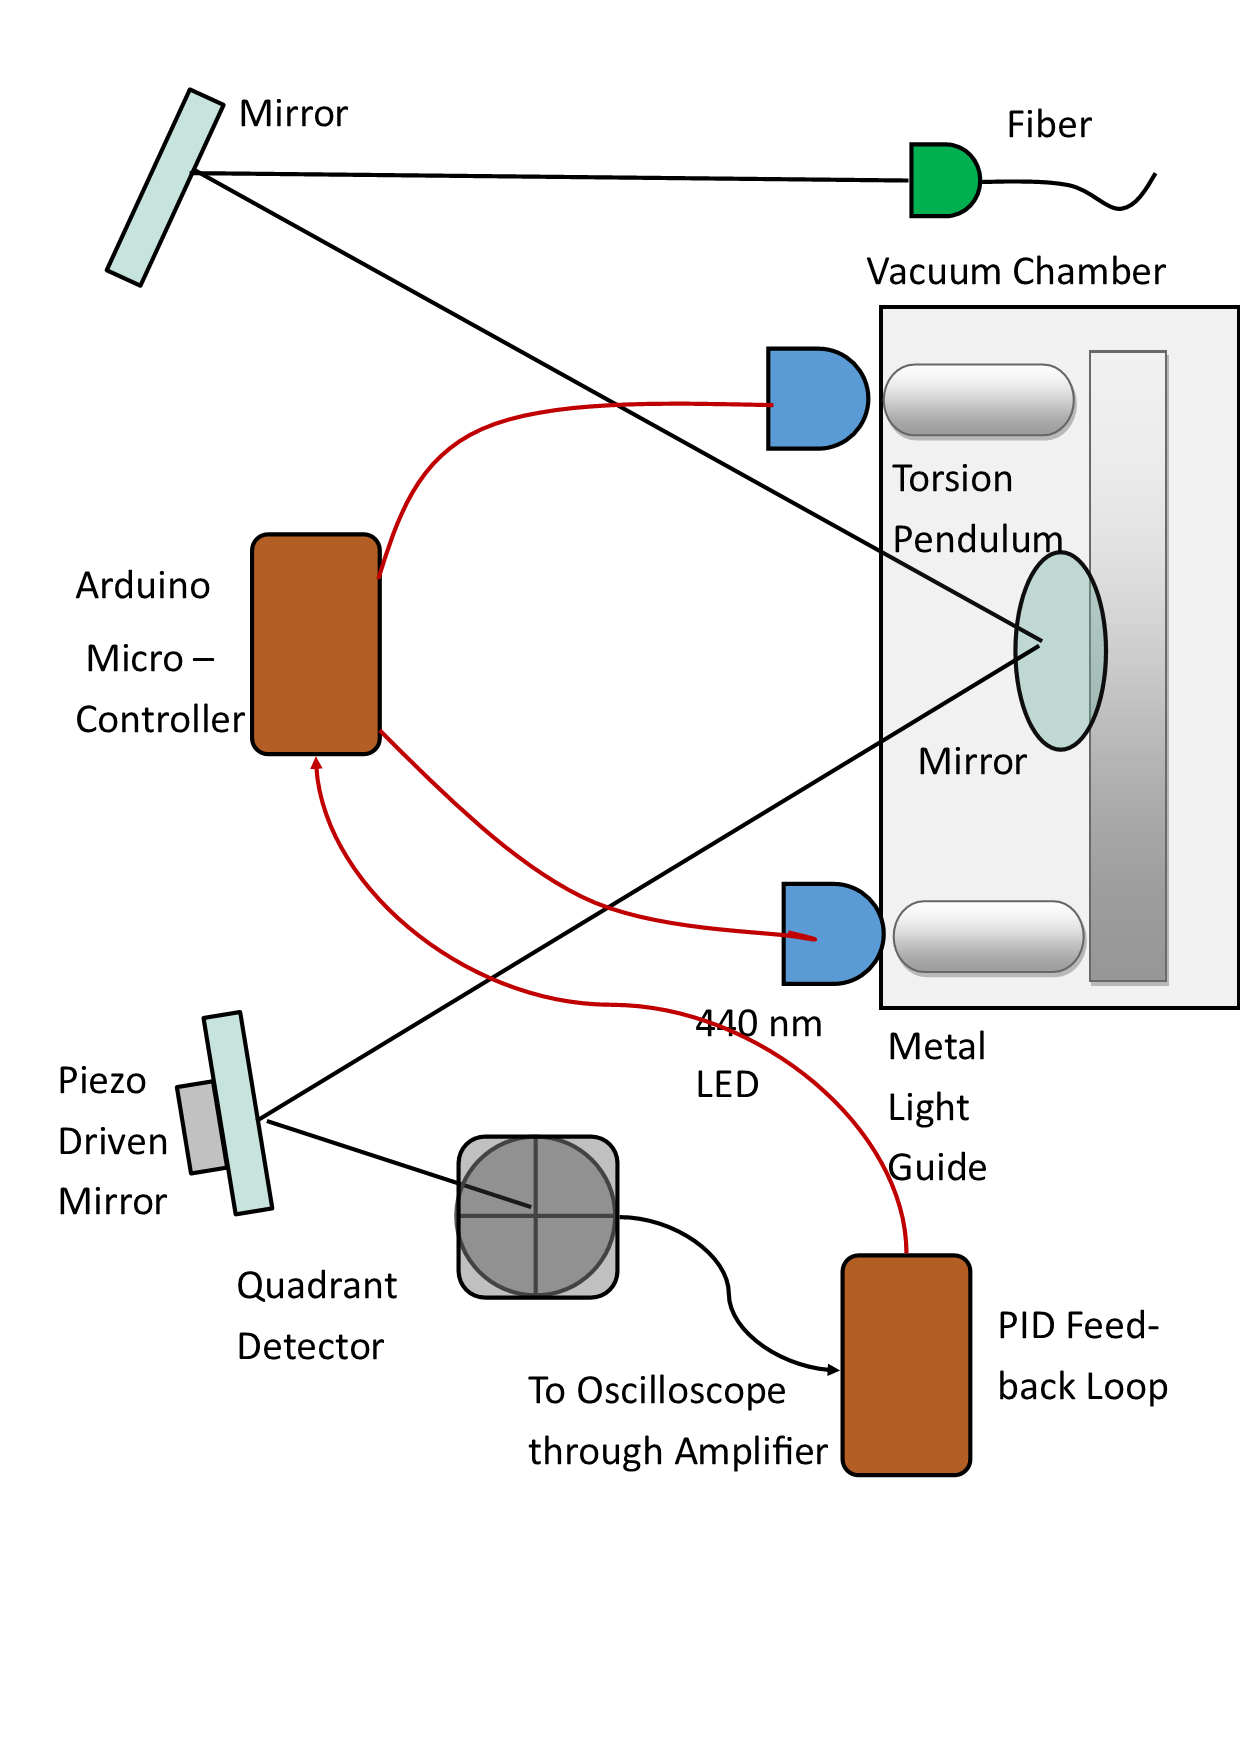
\includegraphics[scale=0.2]{\main/images/4 - methods and results/setup.png}}
	\caption[The experiment setup]{The experiment setup}
	\label{fig:setup}
\end{figure}
\FloatBarrier
\par\noindent
The experiment setup, shown in fig.~\ref{fig:setup}, is composed of a torsion pendulum placed inside a vacuum chamber, a tilt angle measurement system and a feedback system. The experiment setup is placed inside a seismic box, which is not shown in the figure. The angle is measured by a laser beam deflected by the pendulum's front mirror and detected by a quadrant detector. The detector is connected to a computer by an oscilloscope through a signal amplifier. The light reflected from the pendulum mirror is reflected by a piezo driven mirror, which is tuned so that the reflected light would strike the detector's center (the PID needs a reference for error calculations). 
\par\noindent
The feedback system is composed of two LED light sources, modulated in real time by an Arduino micro-controller which is controlled by the PID feed-back loop in the computer. The LED light sources are placed each in front of a transparent windows (viewports) on the sides of the vacuum chamber, each coupled to a side mass of the pendulum. 
\par\noindent
The vacuum chamber is connected to a vacuum engine, which is pumping out the pressure. When the desired pressure is achieved, the vacuum engine is disconnected using the valve and turned off, and the seismic box is closed. When the oscillations settle down to a level which could be affected by the weak torques caused by radiation pressure (an amplitude caused mainly by environmental noises, as explained in previous chapters). The angle is read in real time by the PID algorithm, and an equivalent radiation-pressure torque is exerted by the LED's flux damping down the pendulum noises.
\subsubsection{Design of the system}
\begin{figure}[htbp]
	\centering
	\fbox{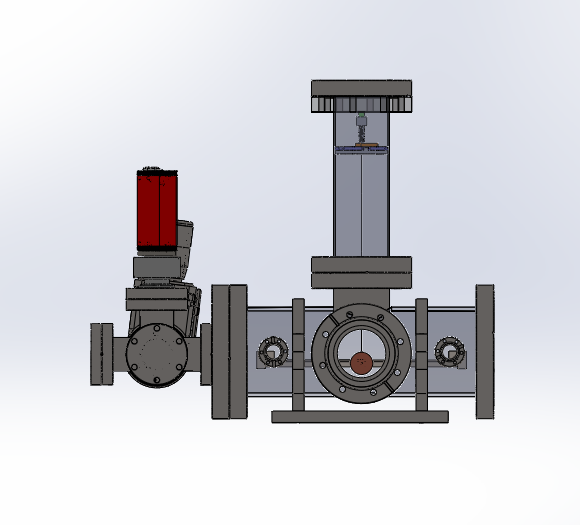
\includegraphics[scale=0.5]{\main/images/4 - methods and results/total_chamber.png}}
	\caption[Total chamber]{The system structure}
	\label{fig:Total chamber}
\end{figure}
\FloatBarrier
\par\noindent
The design of torsional pendulum and vacuum chamber, shown in fig.~\ref{fig:Total chamber}, was carried out using the software Solid Works. The torsional pendulum was manufactured by the university workshop, and the vacuum chamber was manufactured by HTC Vacuum, the assembling was performed at the lab. The system had undergone changes, and the final build of the system is shown. 
\par\noindent
As shown previously (eq.~\ref{eqn:Brownian power}, eq.~\ref{eqn:heat conduction}, eq.~\ref{eqn:acoustic power}, eq.~\ref{eqn:drag force}), Brownian motion energy coupling, thermal coupling, acoustic waves and friction are pressure dependent and are considerably reduced by maintaining low pressure. Therefore, the torsional pendulum is placed inside a vacuum chamber. Magnetic noise is reduced by choosing low magnetic permeability materials, avoiding capacitance and using a Faraday cage. 
\par\noindent
The vacuum chamber is placed inside seismic box, further reducing acoustic waves and magnetic noise. In order to maintain low pressure for long periods, the system is designed to minimize the outgassing rate by both, choosing low outgassing materials and avoiding air pockets inside the devices. 
\subsection{Vacuum chamber design}
\begin{figure}[htbp]
	\centering
	\fbox{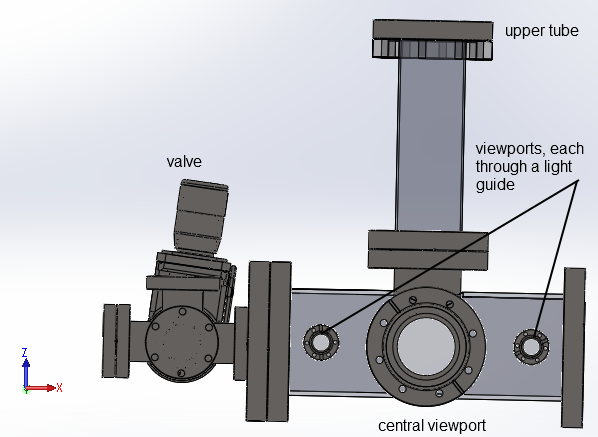
\includegraphics[scale=0.5]{\main/images/4 - methods and results/chamber_front_names.png}}
	\caption[Vacuum chamber, front view]{Vacuum chamber, front view}
	\label{fig:chamber front}
\end{figure}
\FloatBarrier

\par\noindent
The vacuum chamber, shown in fig.~\ref{fig:chamber front}, is composed of two cylindrical tubes placed one over the other with three view ports in front and light guides. The chamber is connected to a vacuum engine and gauge. The vacuum engine is connected to the chamber through a valve. The measurements are conducted when the valve is closed and the engine is off, to prevent rotation noise.

\subsubsection{Chamber viewports}
\par\noindent
The central viewport is located in front of the pendulum's front mirror. The central viewport has a 68.3mm view diameter where the mirror is located 82 mm away, giving a measurement FOV of about $39^0$ degrees. The other two small viewports are located in front of the pendulum's side masses and they are used for damping down the pendulum noises. They are connected to the chamber through light guides. The view ports are transparent for light in 550-1100 nm range, with about 98$\%$ power transmittance in this range. 


\subsubsection{Pressure increase}
\par\noindent
In this experiment, due to the measurement sensitivity, the vacuum engine pumping must be off during measurement. The main limitations to the maintenance of low pressure are the leakage $Q_L$ from the outside (eq.~\ref{eqn:leak rate}) and the outgassing $Q_{des}$ inside the chamber (eq.~\ref{eqn:desorption rate}), thus increase of the pressure at a constant rate over time. Due to the pendulum's shape and size, the vacuum chamber has large volume (high leak rate) and shell area (high outgassing rate).
\par\noindent
In order to minimize the pressure increase rate, the vacuum chamber is built using CF components which are designed for ultra high vacuum, and minimize the leak rate. Also, to reduce outgassing, the torsional pendulum and vacuum chamber were baked-out at $120 C^0$ for a week, using resistive wire. The achieved pressure for the experiments after cooling down is $P \approx 1\cdot 10^{−4} [Hpa]$ for a month without pumping with the vacuum engine.



\subsection{Torsional pendulum design}
\subsubsection{Adjustable mount}
\begin{figure}[htbp]
	\centering
	\fbox{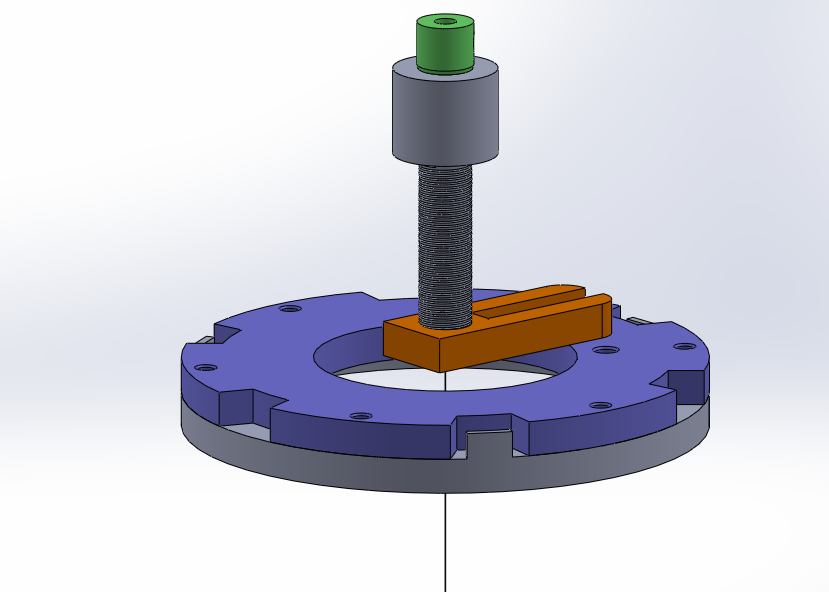
\includegraphics[scale=0.2]{\main/images/4 - methods and results/mount.png}}
	\caption[The pendulum mount]{The pendulum mount}
	\label{fig:mount}
\end{figure}
\FloatBarrier
\par\noindent
An adjustable mount is soldered to the upper tube of the chamber, as shown in fig.~\ref{fig:mount}. The string of the torsional pendulum is held by the mount, enabling to adjust the height, distance and angle of the pendulum relative to the viewports, placing it in front accurately. 
\begin{figure}[htbp]
	\centering
	\fbox{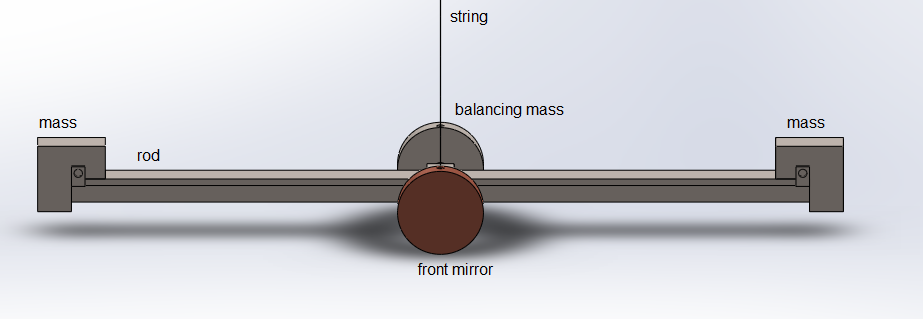
\includegraphics[scale=0.3]{\main/images/4 - methods and results/pendulum_front_names.png}}
	\caption[Torsional pendulum, front view]{Torsional pendulum, front view}
	\label{fig:pendulum front}
\end{figure}
\FloatBarrier
\par\noindent
The torsional pendulum design, shown in fig.~\ref{fig:pendulum front}, is composed of a thin rod with length $2l$, string with length $h$, two identical masses $m$ on the sides, a front mirror and a balancing mass. The mirror is used for tilt angle measurement. Due to an unbalanced center of mass, the earth's gravity causes a downward torque $\tau_y$. 
\begin{figure}[htbp]
	\centering
	\fbox{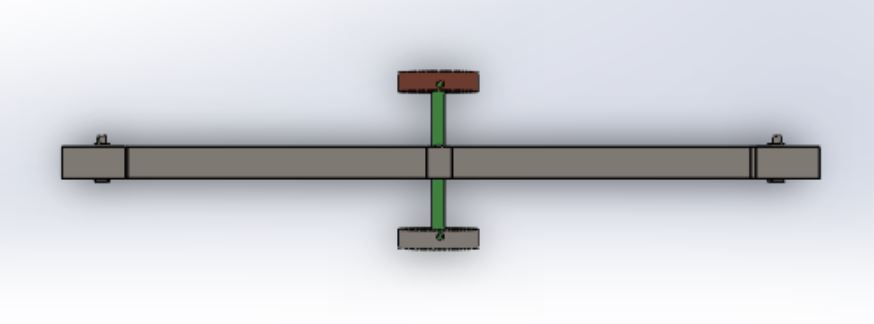
\includegraphics[scale=1.2]{\main/images/4 - methods and results/pendulum_top.JPG}}
	\caption[The torsional pendulum, top view]{The torsional pendulum, top view}
	\label{fig:pendulum top}
\end{figure}
\FloatBarrier 
\par\noindent
The center of mass is balanced using a balancing mass with similar shape and weight as the mirror, as shown in fig.~\ref{fig:pendulum top}. The balancing mass and the mirror are connected to the pendulum by a beam with length $w$ from their centers, and the downward torque is given by:
\begin{equation}
\tau_y = r_1\cdot m_1 g \cdot cos(0) - r_2\cdot m_2 g \cdot cos (0)\ = g( m_1 r_1  - m_2 (w-r_1) )  =0    \label{eqn:downward torque}
\end{equation}
Where $m_1$, $m_2$ are the masses of the mirror and the balancing mass, and $r_1$, $r_2$ are their distance from the pendulum's center of mass respectively. The beam allows to cancel out $\tau_y$ by accurate adjustment of the distance $r_1$, given by: 
\begin{equation}
 r_1 = \frac{w}{\frac{m_1}{m_2}+1}  \label{eqn:downward torque cancelled}
\end{equation}


\subsubsection{Design constraints}
\par\noindent
The chosen pendulum dimensions are designed to achieve large angle sensitivity to torque caused by a the gravity field (small string torsion coefficient $\kappa$ is needed, see eq.~\ref{eqn:theta average}) while maintaining large angle sensitivity to mass (longer oscillation time period $T$, see eq.~\ref{eqn:theta average}). For a torsional pendulum with moment of inertia $I$ and string torsion coefficient $\kappa$, the period $T$ is given by (eq.~\ref{eqn:undamped_omega}): 
\begin{equation}
T = 2\pi\sqrt{\frac{I}{\kappa}}= 2\pi\sqrt{\frac{2ml^2}{\kappa}} =  2\pi\sqrt{\frac{2ml^2}{\frac{G}{h} \frac{\pi d^4}{32}}}  \label{eqn:undamped_motion_equation_4}
\end{equation}
\par\noindent
As shown in eq.~\ref{eqn:undamped_motion_equation_4}, longer string $h$ with smaller diameter $d$ results in small string torsion coefficient while having a large period. A tungsten string is both, vacuum compatible (material with low outgassing) and has high tensile strength \cite{tungsten}, which allows holding the pendulum robustly inside the vacuum chamber while having small string diameter. 
\par\noindent
In order to minimize the magnetic noise in the measurements, the torsional pendulum is made out of stainless steel 316 (instead of stainless steel 304) which has lower magnetic permeability \cite{SS316}, and the chosen front mirror is made fully of oxygen-free copper (OFC) instead of coated glass thus preventing capacitance. 
\subsubsection{Technical information}
The designed elements specifications:
\begin{multicols}{2}
\raggedcolumns
\begin{easylist}
& Torsional beam;
&& Stainless steel 316.
&& length $2l=0.218 [m]$.
&& cross section $A =1.14\cdot10^{-2}[m^2]$.
&& mass weight $m=20.5\cdot10^{-3} [kg]$.
%& Mirror;
%&& OFC, gold coated.
%&& diameter of 1 inch.
\end{easylist}
\columnbreak
\begin{easylist}
& Tungsten string;
&& 99.95\% pure Tungsten
&& shear modulus $G$ of 130-160 Gpa.
&& length $h= 0.249 [m]$.
&& diameter $d=80\cdot10^{-6}[m]$.
\end{easylist}
\end{multicols}



\subsection{Noise reduction}
The measurement system is placed inside a seismic box which is also a Faraday cage with 76 mm thickness, that can block magnetic fields with frequencies $f \ge 30 [Hz]$ from the environment. Thus, the seismic box both reduces acoustic waves and magnetic noise from the environment.
\par\noindent
The vacuum chamber is a second cage that blocks magnetic noise from the electronic system placed inside the seismic box. The vacuum chambers is made out of approximately 3 mm thick stainless steel, blocking magnetic fields with frequencies $f\ge 20 [KHz]$ and reducing magnetic noise with lower frequencies.
\par\noindent
As shown previously, there are environment noises affecting the torsional pendulum (eq.~\ref{eqn:Brownian power}, eq.~\ref{eqn:heat conduction}, eq.~\ref{eqn:acoustic power}, eq.~\ref{eqn: Stefan–Boltzmann power}). Assuming pressure of $P = 1\cdot 10^{−4} [Hpa]$, gas and environment temperature of $T = 298K$ and pendulum temperature $T_0 = 0K$ (maximal noise power), the power of the different noises is given by:
\begin{easylist}
& Black body radiation power $p=0.38[W]$ 
& Thermal flow power $p=0.083[W]$
& Brownian motion power $p=1.2\cdot 10^{-22}[W]$
& Acoustic waves power $p=1.14\cdot 10^{-28}[W]$
\end{easylist}
The black body radiation and heat flow, are temperature dependent and thus grow gradually while the torsional pendulum temperature is reduced. Due to to the remaining noises, the initial oscillations amplitude is $\theta_{max} = 5\cdot10^{-7}[rad]$. 
\subsection{results}
The torsional pendulum parameters:
\begin{multicols}{2}
\raggedcolumns
\begin{easylist}
& expected;
&& $I = 0.487\cdot10^{-3}[kg\cdot m^2]$
&& $\kappa = 2.1\cdot10^{-6}[\frac{N\cdot m}{rad}] - 2.6\cdot10^{-6} [\frac{N\cdot m}{rad}]$
&& $T = 96[s] - 86 [s]$
\end{easylist}
\columnbreak
\begin{easylist}
& measured;
&& $P=1\cdot 10^{−4} [Hpa] $
&& $\kappa = 2.7\cdot10^{-6}[\frac{N\cdot m}{rad}]$
&& $T = 84[s]$
&& $\theta_{max} = 5\cdot10^{-7}[rad]$
\end{easylist}
\end{multicols}
\section{Proportional–Integral–Derivative (PID) controller}
\subsection{Control stability}
A PID feed-back loop is damping the torsional pendulum by continuously calculating the error value of the measured signal from a defined set point $e(t) =SP -\theta(t) $, and damp it to zero. The PID aims to reach the $SP$ with critical damping of the process (the torsional pendulum).
\par\noindent
In control theory there are two wanted conflicting properties; an accurate response (small overshoot), and small risetime (fast response). Overshoot is when the output signal (the actual PID response) exceeds the target value (the wanted response), thus the response is not accurate. The overshoot $PO$ of a second order system is given by:
\begin{equation}
overshoot = 100\cdot e ^{\frac{-\xi\pi}{\sqrt{1-\xi^2}}} = \frac{output-target}{target}   \label{eqn:percentage_overshoot}
\end{equation}
\par\noindent
The PID response to error (shown in eq.~\ref{eqn:PID response}) defines how much will the oscillator overshoot the $SP$. A PID control does not guarantee optimal control or stability of the process. When not tuned correct, it can either overshoot or have a slow response, both resulting with a driven oscillator.
\par\noindent
As seen in eq.~\ref{eqn:percentage_overshoot} when PID gains are too high, instead of critical damping there is overdamping, which is causing overshoot. Due to the high gains the overshoot response overshoots again to the other side, causing the system to be a driven oscillator (shown in eq.~\ref{eqn:driven_motion_equation_2}). A slow response causes phase delay between the signal and the equivalent PID response, again resulting with a driven oscillator.
\subsection{Damped oscillator}
The PID mainly acts as friction, gradually working when the oscillations are at the maximum velocity slowing them down, with a torque $\tau_{PID}$ given by:
\begin{equation}
\tau_{PID}(t) = -\gamma\dot{e}(t) =  -\gamma\cdot [\dot{SP} -\dot{\theta}(t)] =-\gamma\cdot [0-\dot{\theta}(t)]  =  \gamma\dot{\theta}(t)  
\label{eqn:friction_torque_pid}
\end{equation}
\par\noindent
Where $\gamma$ is the PID damping coefficient, since $SP$ is constant, $\dot{e}(t)$ is the the torsional pendulum's oscillations velosity $\dot{\theta}(t)$. The torsional pendulum is a simple harmonic oscillator with initial oscillations amplitude $\theta_{max}$ and velocity amplitude $\dot{\theta}_{max} =\frac{2\pi}{T} \theta_{max}$ (see eq.~\ref{eqn:undamped_motion_equation_solved}). The PID damping coefficient $\gamma$ is given by:
\begin{equation}
\gamma  =  \frac{\tau_{PID}(t)}{\dot{\theta}(t)} = \frac{max(\tau_{PID})}{\dot{\theta}_{max}} =  \frac{max(\tau_{PID})}{\theta_{max}\cdot\frac{2\pi}{T}} =\frac{max(\tau_{PID})}{\theta_{max}}\cdot \frac{ T}{2\pi}          \label{eqn:damped_pid_motion_equation_2}
\end{equation}
Where $max(\tau_{PID})$ is the maximal torque exerted by the PID. When damping using a PID the damping time $\tau$ and damping ratio $\xi$ are given by (eq.~\ref{eqn:damping_time}):
\begin{equation}
\tau = \frac{T}{2 \pi \xi } =  \frac{2I}{\gamma} = \frac{\theta_{max}}{ max(\tau_{PID})} \cdot \frac{4\pi I}{T}  \label{eqn:damping_time_pid}
\end{equation}
The PID damping $\gamma$, damping time $\tau$ and damping type $\xi$ depend on the ratio $\theta_{max}/max(\tau_{PID})$. If $\theta_{max}$ is too large compare to the external torque, the PID affect is negligible, causing an extremely underdamped pendulum with an infinite damping time. When the pendulum is critically damped  by $\tau_{critical}$ (eq.~\ref{eqn:critically_damped_motion_equation}), the damping ratio $\xi$ is given by:
\begin{equation}
\xi = \frac{T^2}{ 8 \pi^2 I }\cdot\frac{ \tau_{critical}}{\theta_{max}} = 1 
\label{eqn:damping_ratio_pid}
\end{equation}
In order to critically damp the torsional pendulum, the PID torque $\tau_{PID}$ needs to be able to exert torques as large as the critical damping torque $max(\tau_{PID}) \geq  \tau_{critical}$, given by:
\begin{equation}
max(\tau_{PID}) \geq  \tau_{critical} = \frac{ 8 \pi^2 I }{T^2}\cdot\theta_{max} = \frac{ 8 \pi^2 \cdot 0.487\cdot10^{-3} }{(86)^2}\cdot 5\cdot10^{-6} = 2.6\cdot10^{-11}[N\cdot m]
\label{eqn:damping_torque_pid}
\end{equation}
\par\noindent
As shown in  eq.~\ref{eqn:damping_torque_pid} the PID maximal torque is given by $max(\tau_{PID}) \geq 2.6\cdot10^{-11}[N\cdot m]$. Since, it is proportional to the oscillations velocity (eq.~\ref{eqn:friction_torque_pid}), it needs a high modulation rate compare to the oscillations period $T$ (to prevent phase delay), and high dynamic range compare to velosity amplitude $\dot{\theta}_{max}$ (to avoid overshoot). 
%The sufficient modulation speed and range are unknown.
\subsection{Radiation-pressure torque}
Two light sources with given flux, $\Theta_i(t)$ cause radiation-pressure forces (eq.~\ref{eqn:radiation_force_power}), one on each mass of the torsional pendulum. As seen in eq.~\ref{eqn:net_gravitation_torque}, the difference between the two torques adds an external net torque. Assuming that both light fields have the same coupling efficiency $\eta$ and are very close to be perpendicular to the surface with negligible incidence angles $\alpha_1\approx\alpha_2\approx 0$, the radiation-pressure net torque $\tau(t)$ is given by:  
\begin{equation}
\tau(t) = l\cdot F_1(t) \cdot cos\alpha_1 - l\cdot F_2(t) \cdot cos\alpha_2\approx l(F_1(t) - F_2(t)) \approx \frac{2l\eta}{{c}} \Delta \Theta(t) \label{eqn:radiation torque}
\end{equation}
The radiation-pressure net torque is modulated by changing the difference between the light sources' flux $\Delta \Theta(t)$. The maximal net torque $\tau_{max}$ is given by: 
\begin{equation}
\tau_{max}  \approx \frac{2l\eta}{{c}} \cdot 2 \Theta_{max} \approx \frac{0.218\cdot \eta}{{3\cdot10^{8}}} \cdot 2 \Theta_{max} \approx 7.27\cdot10^{-10} \cdot \eta\Theta_{max}   \label{eqn:max radiation torque}
\end{equation}
Where $\Theta_{max}$ is the is the the light sources' maximal flux with optical setup efficiency $\eta$. 
\subsection{Laser setup}
Initially the modulated light sources were composed of a single laser diode coupled in series into two acousto optic modulators (AOM), with mod cleaning by coupling the modulated light into the torsional pendulum through optical fibers. An AOM can divide a single coherent light beam into two beams, with intensity ratio proportional to the AOM response to input voltage, resulting with controlled modulation of the light sources difference.
\par\noindent
The apparatus had dynamic range of 1000 steps and modulation speed of $1 sec$. The setup minimized uncertainties of the light intensity since both light sources had a mutual source, partly cancelling internal noises such as thermal and shot noise. 
\par\noindent
The apparatus uncertainty due to the non linearity of the AOM response and laser power fluctuations proved to be larger than the uncertainties of the intensity difference. Also, modulation speed (response time) proved to be more important than modulation range. 
\subsection{Arduino microcontroller}
The modulated light sources are composed of two LED light sources driven by an Arduino microcontroller with a linear response of the LED power to the PID control, causing a linear response of the torque (see eq.~\ref{eqn:radiation torque}) which minimizes the overshoot, and a fast response time which minimizes phase delay.
\par\noindent
The Arduino is an inexpensive open-source microcontroller with a serial communication interface and a digital output without digital-to-analog converter (DAC). The Arduino Mega 2560 contains ATmega2560 8-bit controller, a $16 [MHz]$ crystal oscillator (clock) and 15 PWM outputs pins with digital output of $V_d = 5[V]$.
\begin{figure}[htbp]
	\centering
	\fbox{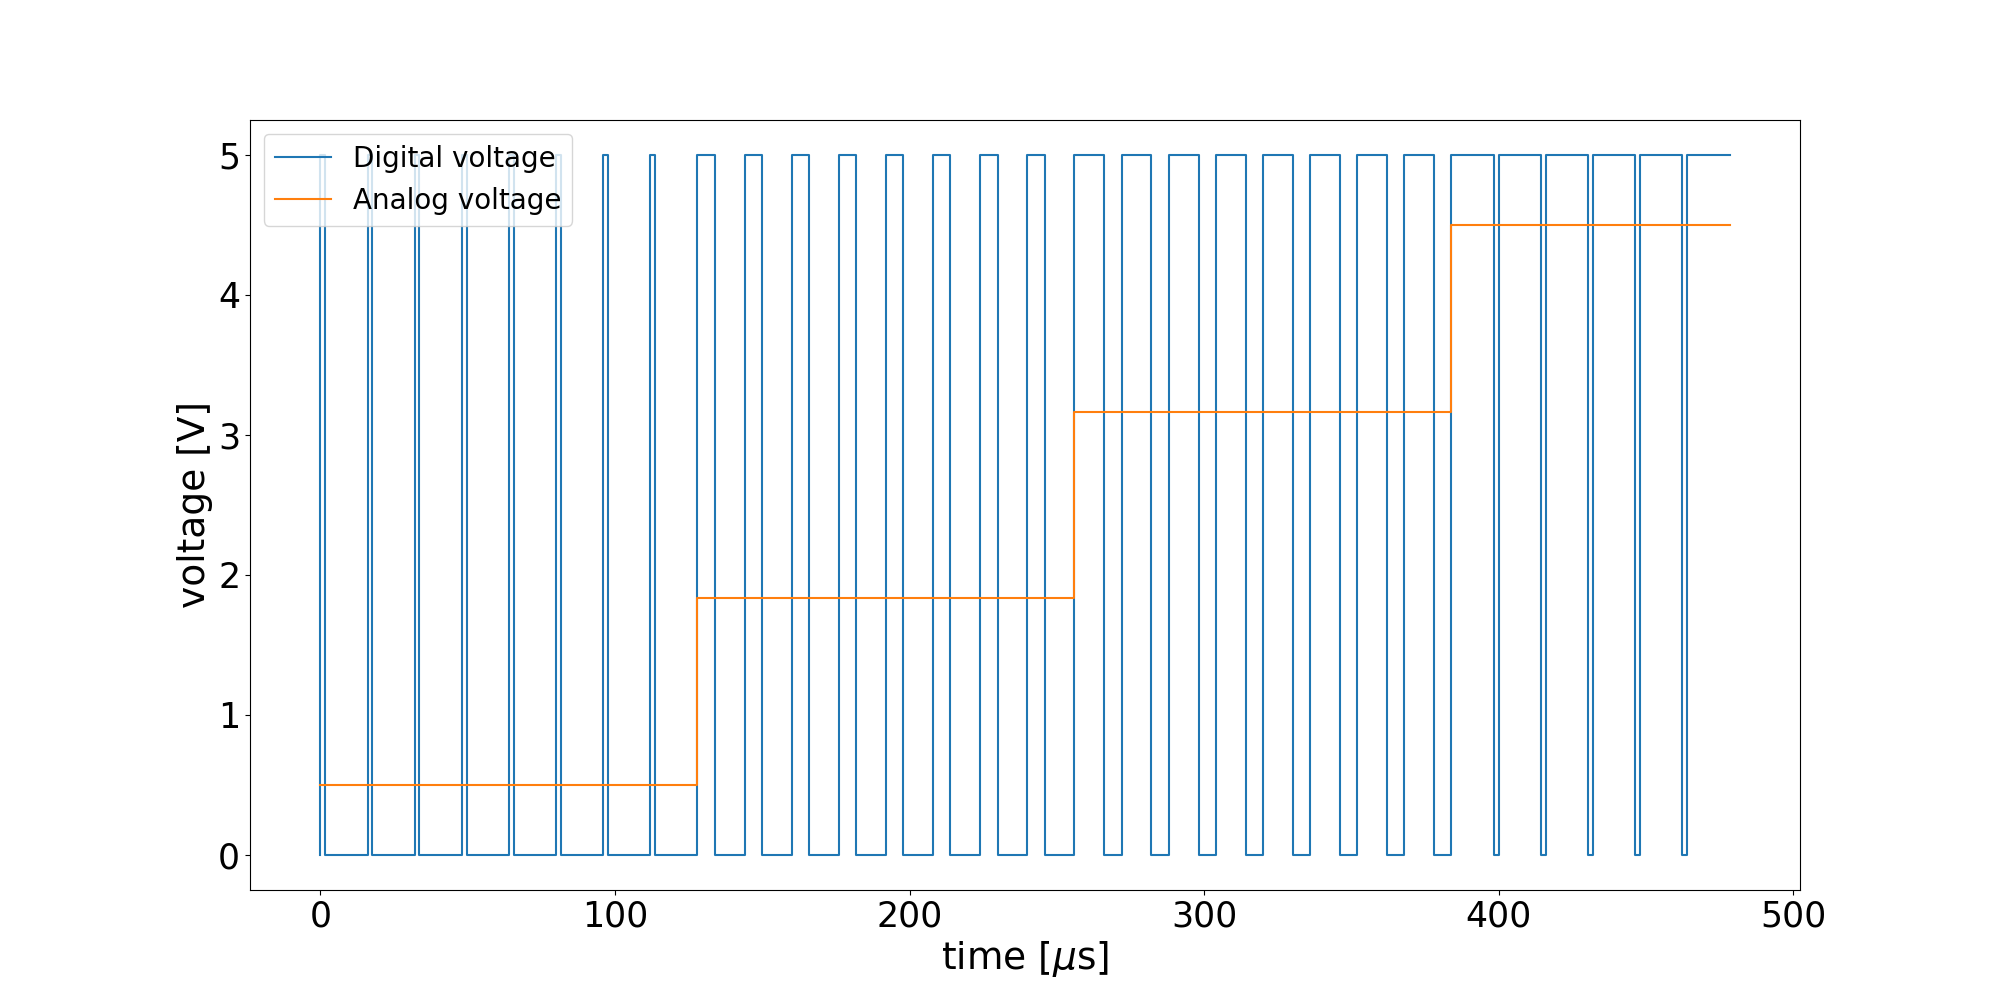
\includegraphics[scale=0.17]{\main/images/4 - methods and results/duty_cycle.png}}
	\caption[The PWM analog voltage]{The PWM analog voltage}
	\label{fig:duty_cycle}
\end{figure}
\FloatBarrier
\par\noindent
The microcontroller can simulate analog output using Pulse Width Modulation (PWM). As shown in fig.~\ref{fig:duty_cycle}, the controller switches the output signal on and off, generating a square wave with period $T$. Pulse width ($PW$) is the time duration in which the signal is on, the controller is able to modulate the $PW$, and thus change the duty cycle which is the ratio of time signal is on compared to off $D(t) = \frac{PW(t)}{T}\cdot 100$. The duty cycle varies between $0-100$, with resolution limited by the controller. The modulation is proportional to the analog average voltage $V_a$ given by: 
\begin{equation}
V_a(t) = \frac{ PW(t)\cdot V_d}{ T}  = \frac{V_d}{100}\cdot D(t)   \label{eqn:pwm voltage}
\end{equation}
Since the Arduino clock is connected to all PWM pins, they are all synchronized and have the same voltage, frequency and phase. The current of $N$ pins connected in parallel is $N\cdot I$.
\par\noindent
Since the clock must have at least 120 periods of square waves before it can change to a new duty cycle value, this limits the voltage modulation frequency. Another limitation to the duty cycle change rate is the controller bit-rate. Accordingly, PWM maximal frequency is given by:
\begin{equation}
f_{PWM} = \frac{1 }{120T}= \frac{1 }{120 \frac{8-bit }{16MHz}}  \approx 500[Hz]	    \label{eqn:pwm frequency}
\end{equation}
\subsection{Light emitting diode (LED)}
The light emitting diode (LED) is a semiconductor light source with high power, and a long lifetime. A forward voltage applied to a p-n junction, causes electron injection which recombine with holes. The recombination releases energy in form of spontaneous emission photons (incoherent light). Due to the electrons life time, the LED could be modulated up to $100MHz$.
\par\noindent
The LED illumination angle varies between $45^0-120^0$. Since emitted light is incoherent it's hard to focus it to a point (not diffraction limited) and it has wide bandwidth spectrum. Given by the Shockley diode equation for p-n junctions, the LED forward voltage $V_l$ is:
\begin{equation}
V_l(I) \approx n V_T ln10 log_{10} (\frac{I}{I_s})\approx constant \label{eqn:led voltage}
\end{equation}
Where $I$ is the LED current, $I_s$ is the saturation current, $n$ is the emission coefficient, and $V_T$ is the thermal voltage. Since the forward voltage varies as the logarithm of the current, it varies slowly, being approximately constant over wide current range, resulting with large changes in the LED current due to small changes in the circuit supply voltage $V$. In the driving circuit a resistor $R$ is connected in series with the LED to stabilizes the current, and the current $I$ is given by:
\begin{equation}
I =\frac{V-V_l}{R} \label{eqn:led circuit}
\end{equation}
\subsection{LED circuit}
The LED is a blue LED with $V_l\approx 4.5V$, $N=6$ parallel PWM Arduino pins for the supply voltage (eq.~\ref{eqn:pwm voltage}) and resistor $R = 200\Omega$. The LED flux $\Theta(t)$ is given by:
\begin{equation}
\Theta(t) = I_{total}\cdot V_l = NI\cdot V_l = N V_l \frac{V-V_l}{R}\cdot  =N V_l\frac{\frac{V_d}{100}\cdot D(t)-V_l}{R} \approx \frac{N V_lV_d}{100R}\cdot D(t) \label{eqn:led power}
\end{equation}
\par\noindent
In order to overcome the LED incoherent profile and large illumination angle, the light sources are coupled to light guides (the vacuum chamber viewports were designed to have light guides in front). A light guide is a pipe made of thin filaments causing internal reflections, designed to illuminate small areas, regardless of the spectral characteristics of the light source. The light guide efficiency is mainly dependent on the cross section and length of the lightguide, making it ideal to overcome focusing problems. 
\par\noindent
Due to coupling efficiency and size difference between the output beam from the lightguide and the pendulum sides, the efficiency of flux hitting the pendulum is estimated $\eta = 0.7$, thus with LED flux given by eq.~\ref{eqn:led power}, the PID torque $\tau_{PID}(t)$ is given by (eq.~\ref{eqn:radiation torque}):
\begin{equation}
\tau_{PID}(t) \approx \frac{2l\eta}{{c}} (\Theta_1(t) -\Theta_2(t)) \approx \frac{2l\eta}{{c}} \cdot\frac{N V_l V_d}{100R}(D_1(t) -D_2(t))  \approx   3.4\cdot 10^{-12}(D_1(t) -D_2(t)) 
\label{eqn:led torque}
\end{equation}
\par\noindent
The torque is controlled by the duty cycle $D(t)$ varying between $0-100$ with 8bit resolution, thus generating torques up to $\tau = 6.8\cdot10^-{10} [N\cdot m]$ with modulation steps of $\Delta\tau = 1.34\cdot10^-{12} [N\cdot m]$ and modulation frequency up to $500[Hz]$ (see eq.~\ref{eqn:pwm frequency}).
\section{Q - factor and results}


\end{document}